
% This LaTeX was auto-generated from an M-file by MATLAB.
% To make changes, update the M-file and republish this document.

\documentclass{article}
\usepackage{graphicx}
\usepackage{color}

\sloppy
\definecolor{lightgray}{gray}{0.5}
\setlength{\parindent}{0pt}

\begin{document}

    
    
\subsection*{Contents}

\begin{itemize}
\setlength{\itemsep}{-1ex}
   \item Ejercicio 6 - Redes neuronales dinámicas
   \item Ejercicio 6.1
   \item entrenarHopfield.m
   \item recuperarHopfield.m
   \item Ejercicio 6.2
   \item Ejercicio 6.3
\end{itemize}


\subsection*{Ejercicio 6 - Redes neuronales dinámicas}

\begin{verbatim}
clear all; close all; clc
\end{verbatim}


\subsection*{Ejercicio 6.1}

\begin{par}
Implemente la arquitectura y entrenamiento Hebbiano para una red recurrente de Hopfield con los patrones que se muestran en la Figura 1.
\end{par} \vspace{1em}
\begin{verbatim}
load('patrones5x5.mat') % cargo los patrones desde un archivo

% Grafico los 3 patrones de la figura 1

N = size(patrones5x5,2);           % cantidad de patrones

invgray = flipud(colormap(gray));  % escala de colores a utilizar
colormap(invgray);                 % blanco y negro

for p = 1:3
    patronReshaped = reshape(patrones5x5(p,:),[5 5]); % patron --> imagen
    subplot(3,3,p); imagesc(patronReshaped'); axis equal tight off
    title('Patron original')
end
\end{verbatim}

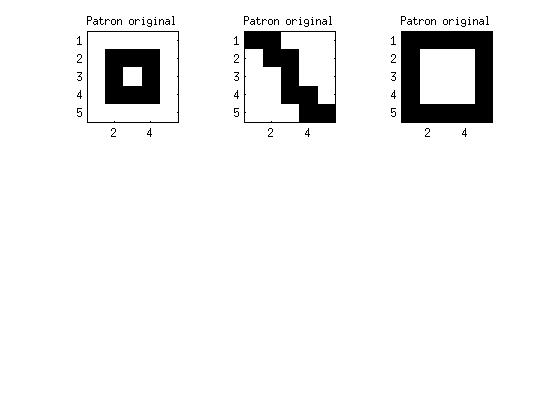
\includegraphics [width=4in]{Ejercicio6_01.png}
\begin{par}
Dados los 3 patrones entreno con ellos una red de Hopfield y obtengo la matriz de pesos.
\end{par} \vspace{1em}
\begin{verbatim}
W = entrenarHopfield(patrones5x5); % matriz de pesos de la red

Pmax = N / (2*log(N));             % capacidad maxima de almacenamiento

fprintf(['La capacidad de almacenamiento %0.2f ' ...
         'supera la cantidad de patrones a recordar (3).\n'], Pmax);
\end{verbatim}

        \color{lightgray} \begin{verbatim}La capacidad de almacenamiento 3.88 supera la cantidad de patrones a recordar (3).
\end{verbatim} \color{black}
    \begin{par}
Ahora pruebo recuperar los patrones originales a partir de patrones ruidosos
\end{par} \vspace{1em}
\begin{verbatim}
cambiar = randperm(N,4); % 4 posiciones que voy a cambiar de signo

for p = 1:3
    ruidoso = patrones5x5(p,:);
    ruidoso(cambiar) = (-1)*ruidoso(cambiar);
    recup = recuperarHopfield(ruidoso, W); % recuperado
    recupReshaped = reshape(recup,[5 5]); % patron --> imagen
    subplot(3,3,6+p); imagesc(recupReshaped'); axis equal tight off
    title('Patron recuperado')
    subplot(3,3,3+p); imagesc(reshape(ruidoso,[5 5])'); axis equal tight off
    title('Patron ruidoso')
end
\end{verbatim}

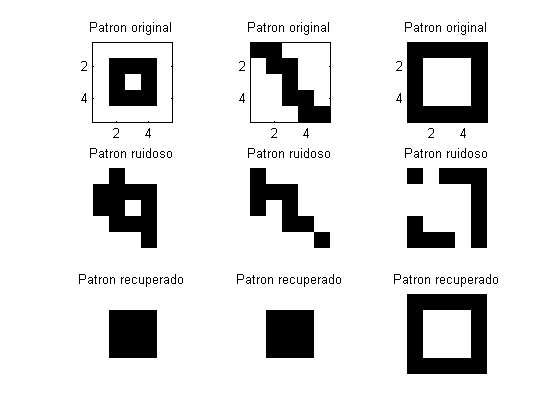
\includegraphics [width=4in]{Ejercicio6_02.png}
\begin{par}
Con el nivel de ruido introducido, 4 cambios en 25 elementos, el segundo y tercer patrón son recuperados en la mayoría de las oprtunidades. En cambio el primer patrón es recuperado con un error en el bit central.
\end{par} \vspace{1em}
\begin{par}
El código de las funciones utilizadas se transcribe a continuación.
\end{par} \vspace{1em}


\subsection*{entrenarHopfield.m}

\begin{verbatim}
dbtype entrenarHopfield.m
\end{verbatim}

        \color{lightgray} \begin{verbatim}
1     function  W = entrenarHopfield( X )
2     % W = entrenarHopfield( X )
3     %   X es una matriz donde cada renglón es un patrón que se desea almacenar.
4     %   W es la matriz de pesos de la red de Hopfield. Dado un patrón, recuerda
5     %     cuales elementos se [des]activaron simultáneamente. 
6     
7     N = size(X,2); % Longitud de cada patron
8     m = size(X,1); % Cantidad de patrones
9     
10    % Entrenamiento Hebbiano
11    % W = x1' * x1 + x2' * x2 + ... + xm' * xm - m * I
12    % La expresión anterior es euivalente a la siguiente
13    W = X' * X - m * eye(N);
14    
15    end
16    

\end{verbatim} \color{black}
    

\subsection*{recuperarHopfield.m}

\begin{verbatim}
dbtype recuperarHopfield.m
\end{verbatim}

        \color{lightgray} \begin{verbatim}
1     function y = recuperarHopfield( y0, W, iterMax, graficar)
2     % y = recuperarHopfield( y0, W, iterMax, graficar)
3     %   y0 es el patrón dado a la entrada, a partir del cuál se recupera y.
4     %      Debe ser un vector fila. 
5     %   W es la matriz de pesos de la red de Hopfield.
6     %   iterMax son las iteraciones máximas permitidas, por defecto son 100.
7     %   graficar es un valor lógico que grafica cada estado intermedio. Por 
8     %      defecto es falso.
9     if nargin < 3
10        iterMax = 100; % iteraciones máximas
11    end
12    if nargin < 4
13        graficar = 0;  % deshabilita la graficación paso por paso
14    end
15    
16    N = length(y0); %
17    iter = 0;       % contador de iteraciones
18    y = y0;         % se inicializa el patrón recuperado igual al patrón dado
19    yant = -y;      % asegura entrar al while sin modificar el algoritmo
20    
21    % Gráfica del patrón de entrada
22    if graficar
23        invgray = flipud(colormap(gray));
24        figure; colormap(invgray)
25        imagesc(reshape(y,[5 5])'); axis equal; axis tight;
26        pause
27    end
28    
29    % El algoritmo itera hasta que el patrón recuperado cumple con y = y * W
30    while (iter < iterMax) && ~isequal(yant, y) 
31        iter = iter + 1;        % contador de iteraciones
32        yant = y;               % se guarda el patrón de la iteración anterior
33        y = sign(yant * W);     % se obtiene el nuevo patrón
34        yEnCero = find(y == 0); % posiciones dónde y se hace cero
35        y(yEnCero) = yant(yEnCero); % si y es 0 se mantiene el anterior valor 
36        
37        % Gráfica del patrón recuperado hasta esta iteración
38        if graficar
39            imagesc(reshape(y,[5 5])'); axis equal; axis tight;
40            pause
41        end
42    end
43    
44    end
45    

\end{verbatim} \color{black}
    

\subsection*{Ejercicio 6.2}

\begin{par}
Utilice la red de Hopfield como memoria asociativa para los patrones de la figura 2.
\end{par} \vspace{1em}
\begin{verbatim}
clear all; figure

load('numeros7x5.mat') % en la posicion 10 se ubica el 0

numMax = 4; % limite de la cantidad de digitos a almacenar
numeros7x5 = numeros7x5(1:numMax,:);% carga los digitos indicados
N = size(numeros7x5,2);             % cantidad de pixeles

invgray = flipud(colormap(gray));  % escala de colores a utilizar
colormap(invgray);                 % blanco y negro

for p = 1:numMax % 10 es 0
    patronReshaped = reshape(numeros7x5(p,:),[7 5]); % patron --> imagen
    subplot(4,numMax,p); imagesc(patronReshaped);
    axis equal tight off
    title('Patron original')
end
\end{verbatim}

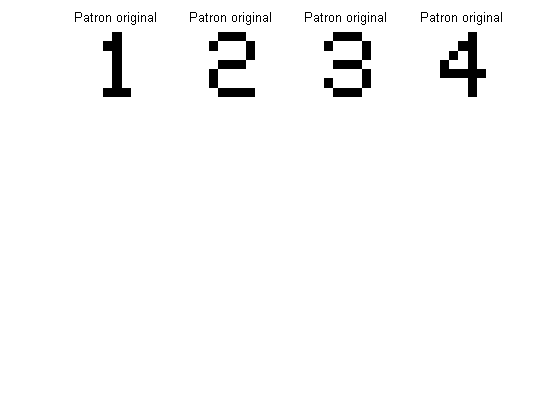
\includegraphics [width=4in]{Ejercicio6_03.png}
\begin{par}
Dados los numMax patrones entreno con ellos una red de Hopfield y obtengo la matriz de pesos.
\end{par} \vspace{1em}
\begin{verbatim}
W = entrenarHopfield(numeros7x5); % matriz de pesos de la red

Pmax = N / (2*log(N));             % capacidad maxima de almacenamiento

fprintf(['La capacidad de almacenamiento es de %0.2f.\n'], Pmax);
\end{verbatim}

        \color{lightgray} \begin{verbatim}La capacidad de almacenamiento es de 4.92.
\end{verbatim} \color{black}
    

\subsection*{Ejercicio 6.3}

\begin{par}
Agregue diferentes cantidades de ruido a los patrones de la Figura 2 y utilice estos ejemplos ruidosos para acceder a las memorias fundamentales almacenadas como en el ejercicio anterior. Para simular cantidades controladas de ruido se sugiere invertir (blanco a negro y viceversa) cada pixel del dígito con probabilidades 0.1, 0.2 y 0.5.
\end{par} \vspace{1em}
\begin{par}
Ahora pruebo recuperar los patrones originales a partir de los patrones con distintos niveles de ruido.
\end{par} \vspace{1em}
\begin{verbatim}
ruidos = [0.1 0.2 0.5]; % niveles de ruido

for p = 1:numMax
    for r = 1:3
        nCambios = floor(N*ruidos(r));
        cambiar = randperm(N,nCambios); % posiciones a cambiar de signo
        ruidoso = numeros7x5(p,:);
        ruidoso(cambiar) = (-1)*ruidoso(cambiar);
        recup = recuperarHopfield(ruidoso, W); % recuperado
        recupReshaped = reshape(recup,[7 5]); % patron --> imagen
        subplot(4,numMax,r*numMax+p); imagesc(recupReshaped);
        axis off equal tight
        tit = sprintf('%2.0f%% ruido',100*nCambios/N);
        title(tit)
    end
end
\end{verbatim}

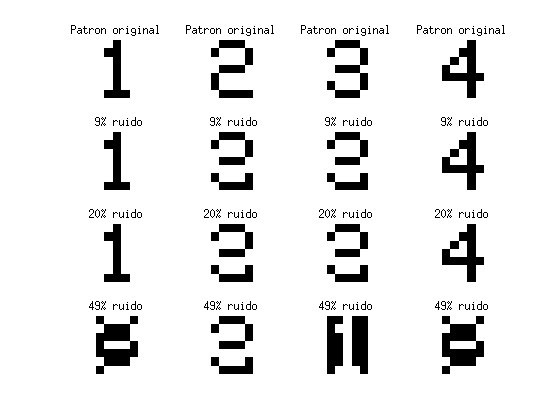
\includegraphics [width=4in]{Ejercicio6_04.png}
\begin{par}
Al entrenar con los 10 números se sobrepasa la capacidad de almacenamiento máxima de la red por lo que se recupera siempre el mismo digito (9) o su versión especular, aún en los niveles de ruidos más bajos.
\end{par} \vspace{1em}
\begin{par}
Reduciendo la cantidad de digitos en la memoria se observa que para cuatro digitos o menos se logra obtener cierto grado de recuperación. Si se entrena con cuatro digitos (como se observa en la Figura NN) se logra recuperar el 1 y el 4, en cambio el 2 y el 3 al ser parecidos devuelven un patrón que se parece a ambos pero no es ninguno de ellos. Con el mayor nivel de ruido (50\%) se pierde toda posibilidad de recuperación.
\end{par} \vspace{1em}



\end{document}
    
